


\begin{frame}
\begin{center}
    \alert<1>{\Huge The Problem} \\ \pause
    \alert<3>{\huge (it's a big one)}\\  %everything is fine meme?
\end{center}

\only<4>{
\begin{figure}[h]
    \begin{center}
    \begin{minipage}{0.45\textwidth}
        \begin{center}
        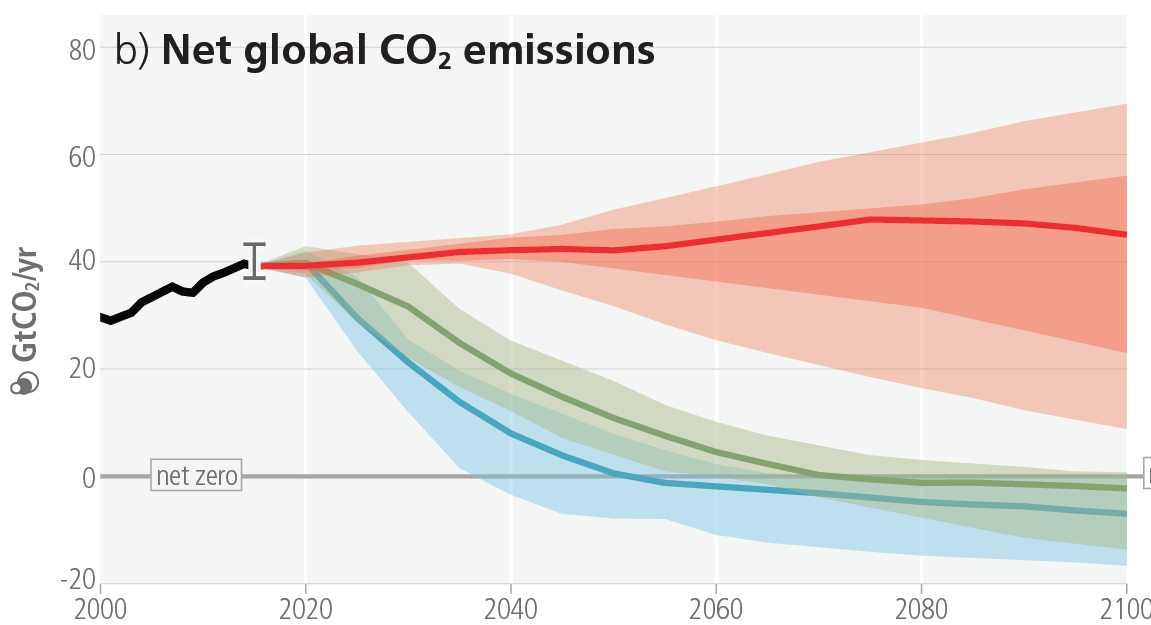
\includegraphics[scale=0.3]{images/CO2IPCC.png}
        \end{center}
    \end{minipage}\hfill
    \begin{minipage}{0.45\textwidth}
        \begin{center}
        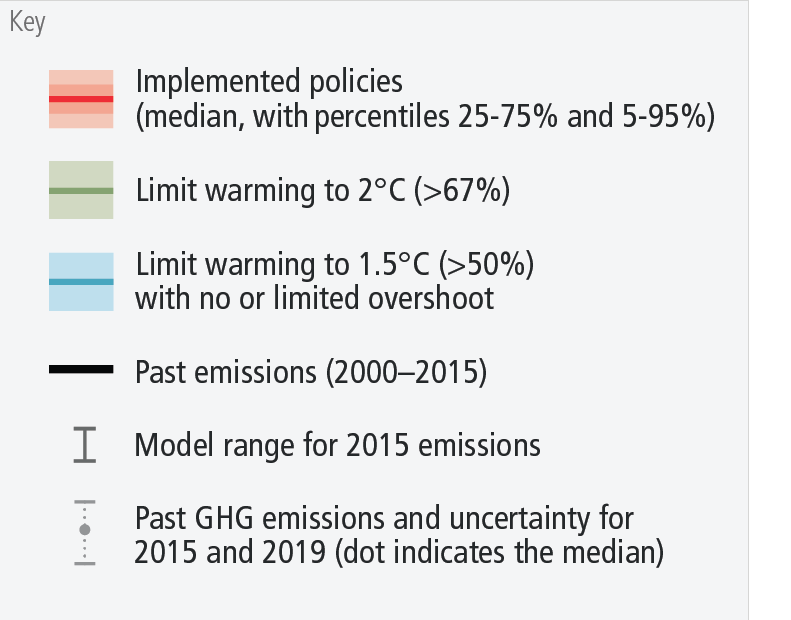
\includegraphics[scale=0.3]{images/legendaIPCC.png}
        \end{center}
    \end{minipage}
    \end{center}
    \caption{CO2 Emissions from the IPCC Report \footnote{IPCC, 2023: Climate Change 2023: Synthesis Report. Available at: \url{https://www.ipcc.ch/report/ar6/syr/}}}
 
\end{figure}

}

\end{frame}
\begin{frame}

\begin{center}
\begin{minipage}{0.7\textwidth}
    \begin{center}
    
\includegraphics[scale=0.5]{images/everythingisfine.jpg}
    \end{center}
\end{minipage}
\end{center}


\end{frame}


\begin{frame}{Energy Grid Transition}

    One of the challenges of transitioning to a fully renewable energy grid comes from two Ducks:
    \\ \bigskip \bigskip
    \pause
    \hspace{3cm}
    \begin{tikzpicture}
        \duckone
    \end{tikzpicture}
    \hspace{4cm}
    \pause
    \begin{tikzpicture}
        \ducktwo
    \end{tikzpicture}
   
\end{frame}

